\chapter{Introduction}\label{chapter:Introduction}
\epigraph{Saving our planet, lifting people out of poverty, advancing economic growth... these are one and the same fight. We must connect the dots between climate change, water scarcity, energy shortages, global health, food security and women's empowerment. Solutions to one problem must be solutions for all.}{\textit{Ban Ki-moon}}

This dissertation considers a way to solve the global problems of energy shortage and environment problem.

\section{Research background and significance}
% 现有太阳能光热发电技术简析,提出太阳能梯级发电的背景及其意义。

% 能源和环境现状
REN21, a global renewable energy policy multi-stakeholder network, published the most comprehensive annual overview of renewable energy of 2016.~\cite{REN21}
Renewables are now established around the world as mainstream sources of energy. Rapid growth, particularly in the power sector, is driven by several factors, including the improving cost-competiveness of renewable technologies, dedicated policy initiatives, better access to financing, energy security and environmental concerns, growing demand for energy in developing and emerging economies, and the need for access to modern energy. 
%An estimated 147 gigawatts (GW) of renewable power capacity was added in 2015.

% 太阳能光热发电现状
Solar energy, which has the advantages of widely distribution, huge amount, inexhaustible and no pollution, has received much attention by many countries and been regarded as the best potential candidate of the fossil energy. The International Energy Agency projected in 2014 that under its "high renewables" scenario, by 2050, solar photovoltaics and concentrating solar power would contribute about 16 and 11 percent, respectively, of the worldwide electricity consumption, and solar would be the world's largest source of electricity.~\cite{IEA2014}

Concentrating solar thermal power generation is another form of power generation technology except solar photovoltaic power generation. Concentrating Solar Power (CSP) energy system uses mirrors to converge sunlight onto a receiver that absorbs the solar energy and transfer it to a heat transfer fluid (HTF) such as a synthetic oil, molten salt or air. The HTF then directly or indirectly used as the heat source in a power cycle.
Compared to solar photovoltaic, solar thermal power is gaining more attention for its advantages as higher energy density, smooth power generation, good grid compatibility, easy to integrate with existing fossil power plant. 

% 文献1
Concentrating solar power technologies use different mirror configurations to concentrate the sun's light energy onto a receiver and convert it into heat. The heat can then be used to create steam to drive a turbine to produce electrical power or used as industrial process heat.
There are three types of CSP technologies being commercialy applied: parabolic trough, parabolic dish and power tower.

A parabolic trough is a type of solar thermal collector whose mirror type is straight in one dimension and curved as a parabola in the other two. The reflector follows the sun during the daylight hours by tracking along a single axis. The energy of sunlight is reflected by the mirror and focused on the pipe positioned at the focal line. HTF (e.g. synthetic oil) runs through the pipe to absorb the heat generated by the focused sunlight, then used as the heat source for heating process or power generation. Figure~\ref{fig:pt} shows a parabolic trough product made by Alpha-E.

\begin{figure}[!ht]
\centering
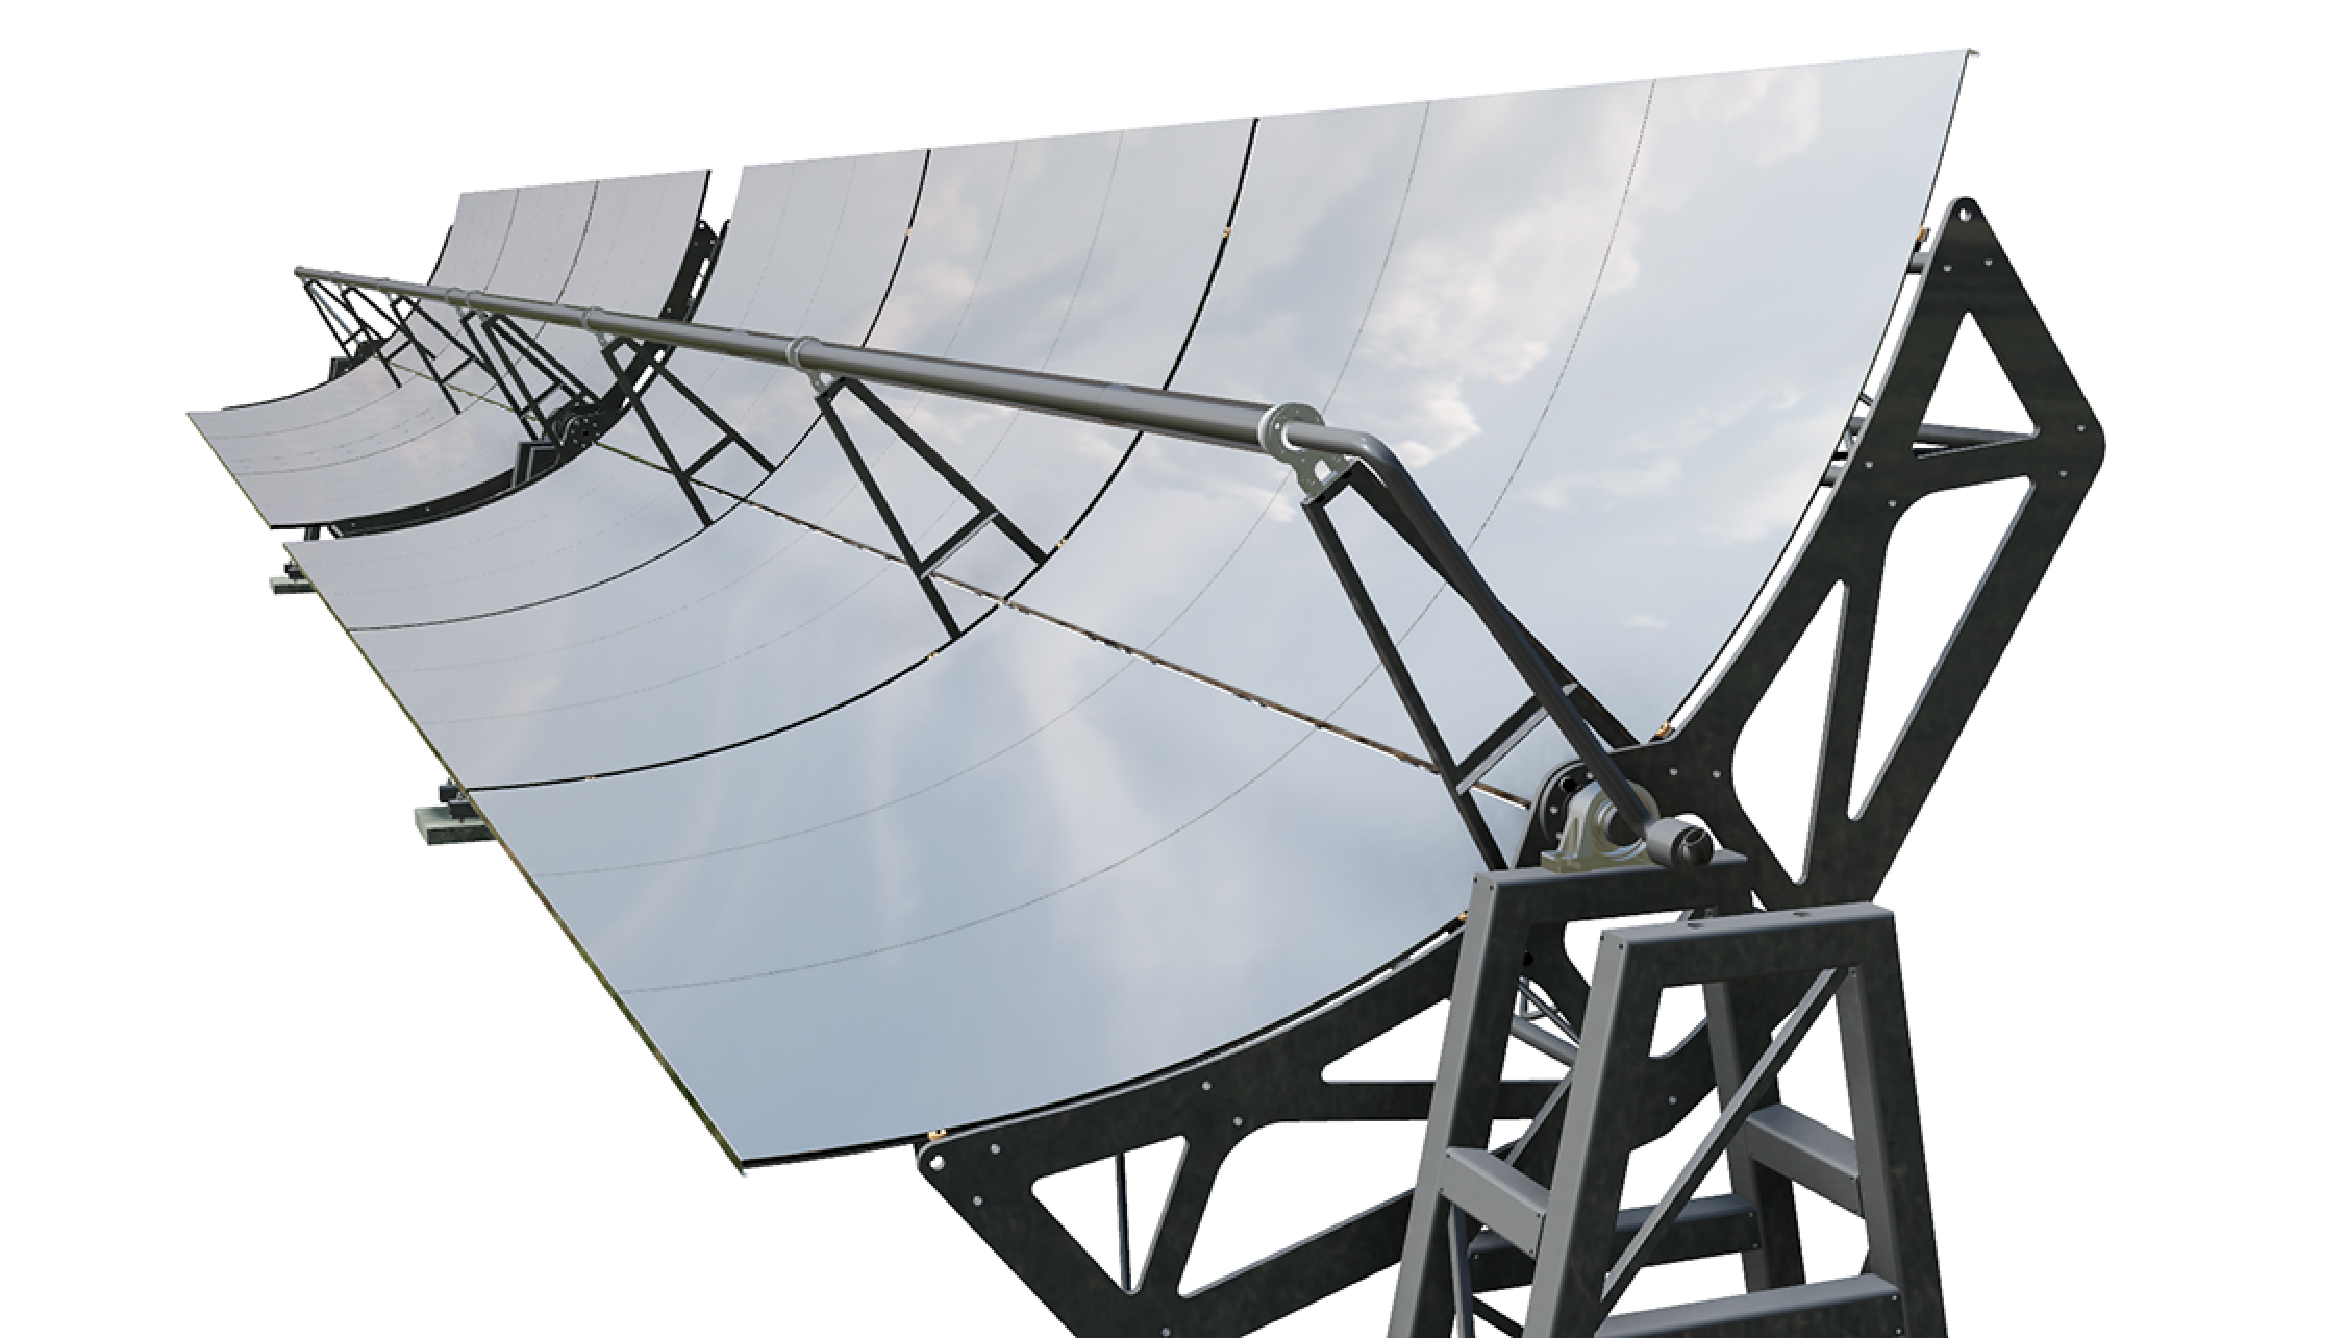
\includegraphics[width=.8\textwidth]{fig/ParabolicTrough}
\caption{Alpha-Trough-350, a parabolic trough product made by Alpha-E}\label{fig:pt}
\end{figure}

A parabolic dish is a type of solar thermal collector whose mirror type is part of a circular paraboloid, that can converging the incoming sunlight traveling along the axis to the focus. A receiver or Stirling engine is put at the focal point to absorb the converged energy. Figure~\ref{fig:pd} shows a 38 kW prototype Stirling engine product of Xiangtan Electric Manufacturing Group Co., Ltd. (XEMC).

\begin{figure}[!ht]
\centering
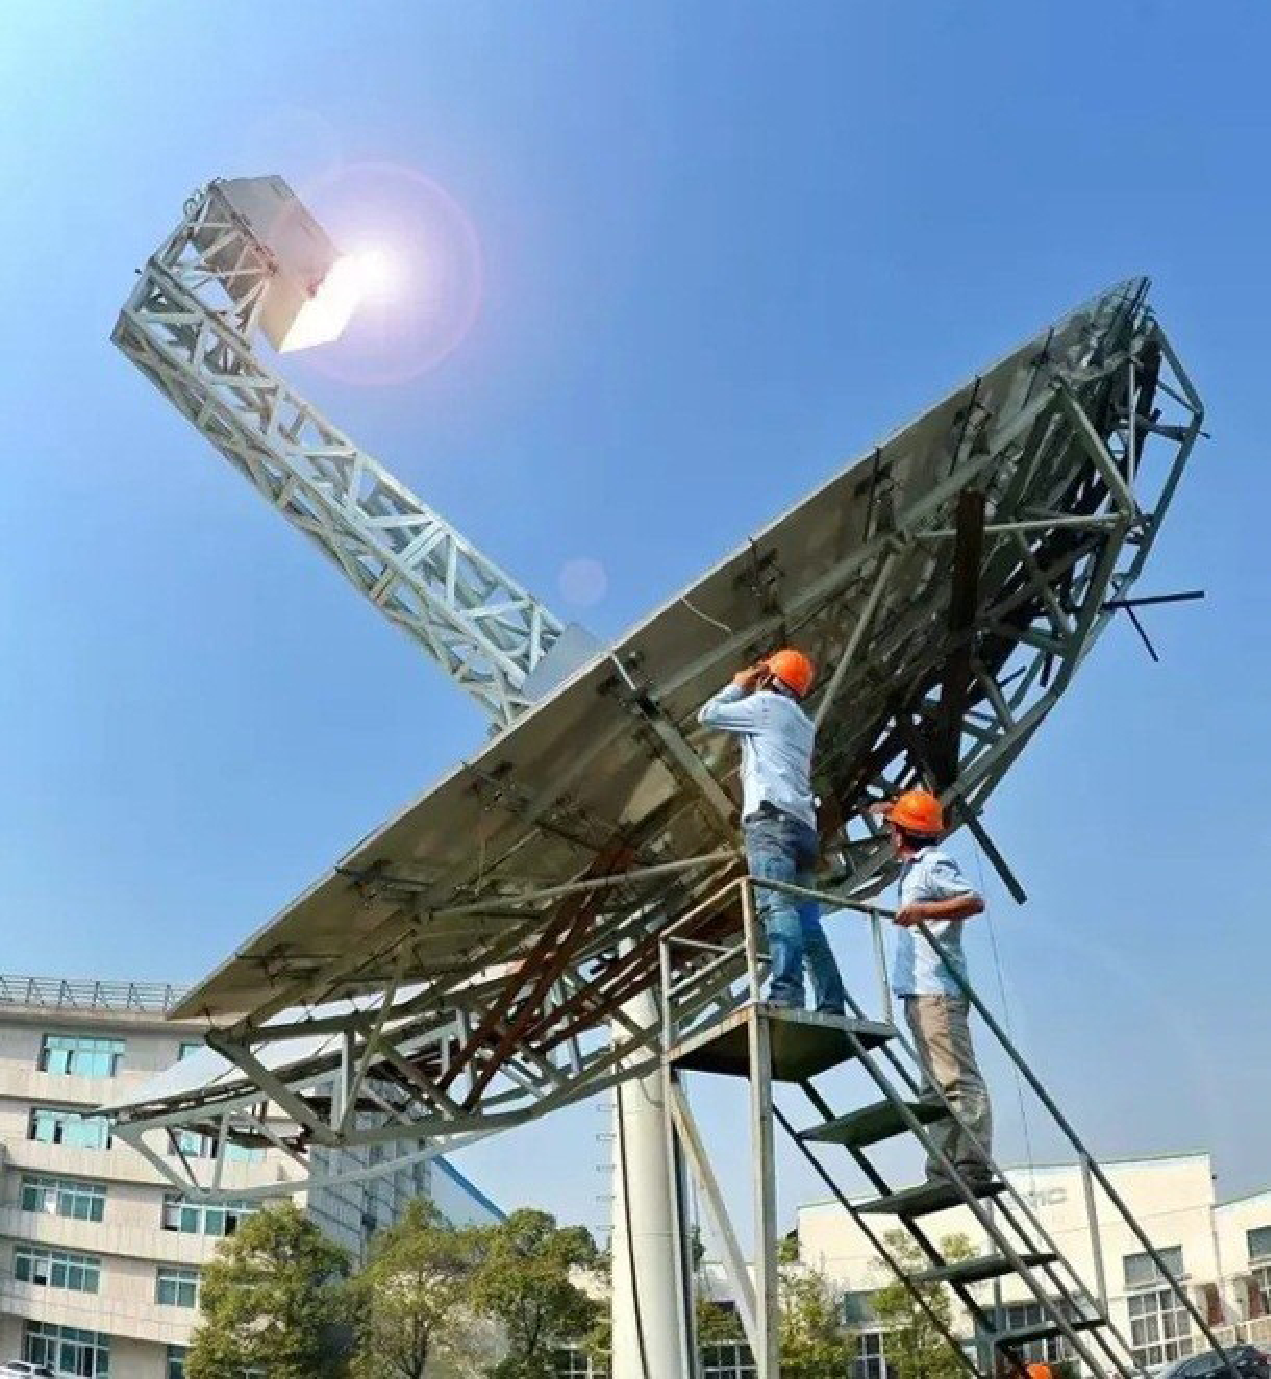
\includegraphics[width=.8\textwidth]{fig/ParabolicDish}
\caption{A 38 kW prototype Stirling engine product of XEMC}\label{fig:pd}
\end{figure}

A solar power tower is a type of solar furnace using a tower to receive the focused sunlight. It uses an array of flat, movable mirrors (called heliostats) to focus the sun's rays upon a collector tower (the target). Figure~\ref{fig:spt} shows the Solar Two power tower.

\begin{figure}[!ht]
\centering
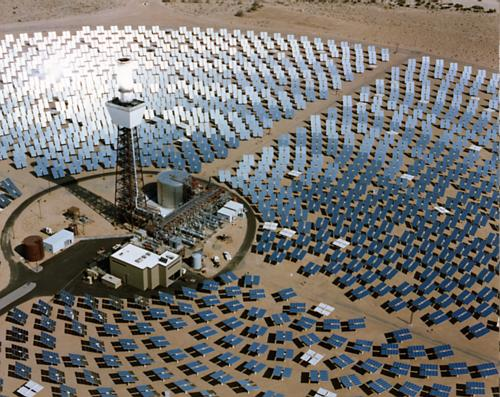
\includegraphics[width=.8\textwidth]{fig/PowerTower}
\caption{Overall view of Solar Two power tower}\label{fig:spt}
\end{figure}

%文献2
%In addition to wind and photovoltaic power, concentrating solar thermal power (CSP) will make a major contribution to electricity provision from renewable energies. Drawing on almost 30 years of operational experience in the multi-megawatt range, CSP is now a proven technology with a reliable cost and performance record. In conjunction with thermal energy storage, electricity can be provided according to demand. To date, solar thermal power plants with a total capacity of 1.3 GW are in operation worldwide, with an additional 2.3 GW under construction and 31.7 GW in advanced planning stage. Depending on the concentration factors, temperatures up to 1000°C can be reached to produce saturated or superheated steam for steam turbine cycles or compressed hot gas for gas turbine cycles. The heat rejected from these thermodynamic cycles can be used for sea water desalination, process heat and centralized provision of chilled water. While electricity generation from CSP plants is still more expensive than from wind turbines or photovoltaic panels, its independence from fluctuations and daily variation of wind speed and solar radiation provides it with a higher value. To become competitive with mid-load electricity from conventional power plants within the next 10–15 years, mass production of components, increased plant size and planning/operating experience will be accompanied by technological innovations. On 30 October 2009, a number of major industrial companies joined forces to establish the so-called DESERTEC Industry Initiative, which aims at providing by 2050 15 percent of European electricity from renewable energy sources in North Africa, while at the same time securing energy, water, income and employment for this region. Solar thermal power plants are in the heart of this concept.
% 现有发电技术的优缺点
% 梯级发电的意义

Among the three solar thermal power technologies, parabolic trough is the most mature and commercially deployed technology. However, it has a low concentration ratio, the receiver's temperature is relatively low, the solar-to-electric efficiency is relatively low. Parabolic dish can obtain high temperature thermal energy, it's solar-to-electric can be higher than parabolic trough.
Besides, one advantage of parabolic trough is that it requires much less water for power generation. However, solar parabolic dish is not a large-scale application, it's mainly applied for distributed power generation for its compact structure and easy installation. Solar power tower has a very high concentration ratio when more mirrors (also called heliostats) are used, the receiver's temperature can be very high and it can be applied for large-scale application. However, it has some disadvantages such as high investment. It is currently in rapid development stage.

It is very important to find out a way the utilize the advantages of existing solar thermal power technologies and overcome their disadvantages. In other words, to find out a new technology with higher efficiency lower cost is urgent.
This research is trying to achieve this by proposing a cascade system that uses different collector power generation methods and different thermodynamic cycles, which may be a new and feasible technology to realize large-scale solar thermal power generation.

\section{State of the art}
% 范围的大小
%国内外对太阳能光热发电技术的研究现状。
%外文文献-问题-解决方案-本项目需求

\subsection{Parabolic trough}\label{sec:pt}

Parabolic trough solar technology is the most proven and lowest cost large-scale solar power technology available.~\cite{Price2002}

Padilla~\cite{Padilla2011} performed a detailed one dimensional numerical heat transfer analysis of a PTC (Parabolic Trough Collector). To solve the mathematical model of heat transfer of the PTC model, the partial differential equations were discretized and the nonlinear algebraic equations were solved simultaneously. The numerical results was validated to the data from Sandia National Laboratory (SNL).
\nomenclature[C]{PTC}{Parabolic Trough Collector}
\nomenclature[C]{SNL}{Sandia National Laboratory}

To understand the thermal performance of the collector and identify the heat losses from the collector, Mohamad~\cite{Mohamad2014} analyzed the temperature variation of the working fluid, tube and glass along the collector.

Guo~\cite{JiangfengGuo2016-1} investigated the energy efficiency and exergy efficiency of the parabolic trough collector. The result shown that there exists an optimal mass flow rate of working fluid for exergy efficiency, and the thermal efficiency and exergy efficiency have opposite changing tendencies under some conditions.

Guo~\cite{JiangfengGuo2016-2} implemented a multi-parameter optimization of parabolic trough solar receiver based on genetic algorithm where Exergy and thermal efficiencies were employed as objective function.

Padilla~\cite{Padilla2014} performed a comprehensive exergy balance of a parabolic trough collector based on the previous heat transfer model~\cite{Padilla2011}. The results shown that inlet temperature of heat transfer fluid, solar irradiance, and vacuum in annulus have a significant effect on the thermal and exergetic performance, but the effect of wind speed and mass flow rate of heat transfer fluid is negligible. It was obtained that inlet temperature of heat transfer fluid cannot be optimized to achieve simultaneously maximum thermal and exergetic efficiency because they exhibit opposite trends. Finally, it was found that the highest exergy destruction is due to the heat transfer between the sun and the absorber while for exergy losses is due to optical error.

Huang~\cite{Huang2012} proposed an analytical model for optical performance which employed a modified integration algorithm.

Wang~\cite{Wang2016} proposed a mathematical model for the optical efficiency of the parabolic trough solar collector and selected three typical regions of solar thermal utilization in China for the model. The model is validated by comparing the test results in parabolic trough power plant, with relative error range of 1\% to about 5\%.

Al-Sulaiman~\cite{AlSulaiman2014} presented the exergy analysis of selected thermal power systems driven by PTSCs. The power pf the thermal power system is produced using either a steam Rankine cycle (SRC) or a combined cycle, in which the SRC is the topping cycle and an organic Rankine cycle (ORC) is the bottoming cycle.
\nomenclature[C]{SRC}{Steam Rankine Cycle}
\nomenclature[C]{ORC}{Organic Rankine Cycle}

Hachicha~\cite{Hachicha2013} presented a detailed numerical heat transfer model based on the finite volume method for the parabolic trough collector.  This model is based on finite volume method and ray trace techniques and takes into account the finite size of the Sun.  The model is thoroughly validated with results from the literature and it shows a good agreement with experimental and analytical results.

Ashouri~\cite{Ashouri2015} coupled a small scale parabolic trough collector and a thermal storage tank along with an auxiliary heater to a Kalina cycle to study the performance of the system throughout the year, both thermodynamically and economically.

Guo~\cite{SuGuo2016} developed a nonlinear distribution parameter model to model the dynamic behaviors of direct steam generation parabolic trough collector loops under either full or partial solar irradiance disturbance.

Bader~\cite{Bader2015} developed a numerical model of a tubular vavity-receiver that uses air as the heat transfer fluid. Four different receiver configurations are considered, with smooth or V-corrugated absorber tube and single- or double-glazed aperture window. The different types of energy loss by the collector have been quantified, and the temperature distribution inside the receiver has been studied. The pumping power required to pump the HTF through the receiver has been determined for a 200 m long collector row.

Good~\cite{Good2015} proposed solar trough concentrators using air as heat transfer fluid at operating temperatures exceeding $600\,^\circ$C. It consists of an array of helically coiled absorber tubes contained side-by-side within an insulated groove having a rectangular windowed opening. Secondary concentrating optics are incorporated to boost the geometric concentration ratio to 97$\times$.

Boukelia~\cite{Boukelia2016} investigated the feed-forward back-propagation learning algorithm with three different variants; Levenberge Marguardt (LM), Scaled Conjugate Gradient (SCG), and Pola-Ribiere Conjugate Gradient (PCG), used in artificial neural network (ANN) to find the best approach for prediction and techno-economic optimization of parabolic trough solar thermal power plant (PTSTPP) integrated with fuel backup system and thermal energy storage.
\nomenclature[C]{LM}{Levenberge Marguardt}
\nomenclature[C]{SCG}{Scaled Conjugate Gradient}
\nomenclature[C]{PCG}{Pola-Ribiere Conjugate Gradient}
\nomenclature[C]{ANN}{Artificial Neural Network}
\nomenclature[C]{PTSTPP}{Parabolic Trough Solar Thermal Power Plant}

Kaloudis~\cite{Kaloudis2016} investigated a PTC system with nanofluid as the HTF in terms of Computational Fluid Dynamics (CFD). Syltherm 800 liquid oil was used as the HTF, and Al$_2$O$_3$ nanoparticles with the concentrations ranges from 0\% to 4\% was investigated. A boost up to 10\% on the collector efficiency was reported for Al$_2$O$_3$ concentration of 4\%.
\nomenclature[C]{HTF}{Heat Transfer Fluid}
\nomenclature[C]{CFD}{Computational Fluid Dynamics}

Tan~\cite{Tan2014} proposed a two-stage photovoltaic thermal system based on solar trough concentration is proposed, in which the metal cavity heating stage is added on the basis of the PV/T stage, and thermal energy with higher temperature is output while electric energy is output. The experimental platform of the two-stage photovoltaic thermal system was established, with a 1.8 m$^2$ mirror PV/T stage and a 15 m$^2$ mirror heating stage, or a 1.8 m$^2$ mirror PV/T stage and a 30 m$^2$ mirror heating stage. The results showed that with single cycle, the long metal cavity heating stage would bring lower thermal efficiency, but temperature rise of the working medium is higher, up to 12.06$\,\circ$C with only single cycle. With 30 min closed multiple cycles, the temperature of the working medium in the water tank was 62.8$\,\circ$C, with an increase of 28.7$\,\circ$C, and thermal energy with higher temperature could be output.

Al-Sulaiman~\cite{AlSulaiman2012} proposed a novel system based on PTC and ORC for combined cooling, heating and power (CCHP). Performance assessment, including efficiency, net electrical power, and electrical to heating and cooling ratios, of the system shown that when CCHP is used, the efficiency increases significantly. This study reveals that the maximum electrical efficiency for the solar mode is 15\%, for the solar and storage mode is 7\%, and for the storage mode is 6.5\%. The maximum CCHP efficiency for the solar mode is 94\%, for the solar and storage mode is 47\%, and for the storage mode is 42\%.
\nomenclature[C]{CCHP}{Combined cooling, heating and power}

Lobon~\cite{Lobon2014} introduced a computational fluid dynamic simulation approach to predict the behavior of a solar steam generating system, which is located at the Plataforma Solar de Almeria, Spain. The CFD package STAR-CCM+ code has been used to implement an efficient multiphase model capable of simulating the dynamics of the multiphase fluid in parabolic-trough solar collectors. Numerical and experimental data are compared in a wide range of working conditions.
\nomenclature[C]{DSG}{Direct Steam Generation}

Xu~\cite{Xu2014} presented a method to compensate the end loss effect of PTC. An optical analysis on the end loss effect of PTC with horizontal north-south axis (PTC-HNSA) is performed and a five-meter PTC-HNSA experimental system was built. The increased thermal efficiency of the experimental system is measured, and the result that the experimental value (increased thermal efficiency) substantially agreed with the theoretical value (increased optical efficiency) is gained.

Liu~\cite{Liu2012} developed a mathematical model of PTC using the least squares support vector machine (LSSVM) method. Numerical simulations are implemented to evaluate the feasibility and efficiency of the LSSVM method, where the sample data derived from the experiment and the simulation results of two solar collector systems with 30 m$^2$ and 600 m$^2$ solar fields, and the complicated relationship between the solar collector efficiency and the solar flux, the flow rate and the inlet temperature of the heat transfer fluid (HTF) is extracted.
\nomenclature[C]{LSSVM}{Least squares support vector machine}

\subsection{Parabolic dish}\label{sec:pd}

One of the main goals of the BIOSTIRLING-4SKA project, funded by the European Commission, is the development of a hybrid Dish-Stirling system based on a hybrid solar-gas receiver, which has been designed by the Swedish company Cleanergy~\cite{Blazquez2016}.

Craig~\cite{Craig2016b} proposed two types of cooking sections of the solar parabolic dish system: the spiral hot plate copper tube and the heat pipe plate. A conical cavity of copper tubes were put on the focus of the collectors to collect heat and the heat is stored inside an insulated tank which acts both as storage and cooking plate. The use of heat pipes to transfer heat between the oil storage and the cooking pot was compared to the use of a direct natural syphon principle which is achieved using copper tubes in spiral form like electric stove. An accurate theoretical analysis for the heat pipe cooker was achieved by solving the boiling and vaporization in the evaporator side and then balancing it with the condensation and liquid-vapor interaction in the condenser part while correct heat transfer, pressure and height balancing was calculated in the second experiment. The results show and compare the cooking time, boiling characteristics, overall utilization efficiencies and necessary comparison between the two system and other existing systems.

Flux distribution of the receiver is simulated successfully by Mao~\cite{Mao2014b} using MCRT method. The impacts of incident solar irradiation, aspect ratio (the ratio of the receiver height to the receiver diameter), and system error on the radiation flux of the receiver are investigated.
\nomenclature[C]{MCRT}{Monte Carlo Ray Tracing}

Mawire~\cite{Mawire2014} investigated the thermal performance of a cylindrical cavity receiver for an SK-14 parabolic dish concentrator. The receiver exergy rates and efficiencies are found to be appreciably smaller than the receiver energy rates and efficiencies. The exergy factor is found to be high under conditions of high solar radiation and under high operating temperatures. An optical efficiency of around 52\% for parabolic dish system is determined under high solar radiation conditions.

Reddy~\cite{Reddy2015,Reddy2015_2} performed the theoretical thermal performance analysis of a fuzzy focal solar parabolic dish concentrator with modified cavity receiver. Total heat loss from the modified cavity receiver is estimated considering the effects of wind conditions, operating temperature, emissivity of the cavity cover and thickness of insulation. Time constant test was carried out to determine the influence of sudden change in solar radiation at steady state conditions. The daily performance tests were conducted for different flow rates.

Vikram~\cite{Vikram2015} investigated the total heat losses of modified cavity receiver of SPD with three configurations using 3D numerical model. The effects of various parameters such as diameter ratio, angle of inclination, operating temperature, insulation thickness and emissivity of the cavity cover on the heat losses from the modified vavity receiver are investigated. An ANN model is developed to predict the heat loss for a large set of influencing parameters. Based on ANN modeling, improved Nusselt number correlations are proposed for convective, radiative and total heat losses from the modified cavity receiver. The convective heat losses are greatly influenced by receiver inclination whereas the radiation heat losses are influenced by the cavity cover emissivity. The diameter ratio also plays a major role in heat losses from the cavity receiver. The present method predicts the heat losses more accurately compared with the existing models.

Atul~\cite{Atul2015} proposed a low-cost solar dish water heating system and investigated the effect of variation of mass flow rate on performance of the heater prototype. A novel truncated cone-shaped helical coiled receiver made up of copper is put at the focal point of SP.

CRTEn developed a solar parabolic concentrator (SPC) using four types of absorbers: flat plat, disk, water calorimeter and solar heat exchanger.~\cite{Skouri2013} For the system different types of absorbers, experiments were conducted to obtain the mean concentration ratio and both energy and exergy efficiency. Results shown that thermal energy efficiency of the system varies from 40\% to 77\%, the concentrating system reaches an average exergy efficiency of 50\% and a concentration factor around 178.
\nomenclature[C]{CRTEn}{Research and Technologies Centre of Energy in Borj Cedria}
\nomenclature[C]{SPC}{Solar parabolic concentrator}

Blazquez~\cite{Blazquez2016} studied the optimization of the concentrator and receiver cavity geometry of parabolic dish system. Ray-tracing analysis has been performed with the open source software Tonatiuh, a ray-tracing tool specifically oriented to the modeling of solar concentrators.

Uma~\cite{Uma2015} carried out the simulation of the structural, thermal and CFD analysis of the dish with varying metallic properties (Aluminium, Copper and StainlessSteel) under different wind conditions. Computational Fluid Dynamics (CFD) was done to simulate the thermal performance of the dish at two different wind velocities.

Patil~\cite{Patil2016} described the development of automatic dual axis solar tracking system for solar parabolic dish. Five light dependent resistors were used to sense the sunlight and Two permanent magnet DC motors are used to move the solar dish. A controller software were developed to control the motors using the data sensed by the resistors.

Pavlovic~\cite{Pavlovic2014} presented a procedure to design a square facet concentrator for laboratory-scale research on medium-temperature thermal processes. A parabolic collector made up of individual square mirror panels (facets) were investigated. These facets can deliver up to 13.604 kW radiative power over a 250$\,\mathrm{mm}$ radius dish receiver with average concentrating ratio exceeding 1200.

\subsection{Power tower}\label{sec:st}

Besarati and Yogi~\cite{Besarati2014} developed a new and simple method to improve the calculation speed and accuracy for shading and blocking computation of the heliostat field. The Sassi method~\cite{Sassi1983} is used for the shading and blocking efficiency. A 50$\,\mathrm{MWth}$ heliostat field in Dagget, California, USA was used as a case study for the proposed method. 

Haroun~\cite{El2015} proposed a novel system combines both solar chimney and solar tower. The solar tower receiver was installed at the top of the chimney. Theoretical study of this novel system was conducted. The results shown that the new system generates more power than conventional system with the same parameters of solar irradiance, collector radius, height of chimney, and height of solar tower. The inlet air speed of the chimney is higher than that of the conventional, and it increases with the solar irradiance. Moreover, the results indicated that there exists a optimum ratio of solar tower height to solar chimney height for the maximum overall power.

Franchini et al.~\cite{Franchini2013} developed a computing procedure for solar tower system under both nominal and part load conditions. A Siemens gas turbine product, SGT-800, was considered as a study case for the solar tower system. The turbine has a dual pressure heat recovery steam generator, which can be used for the Integrated Solar Combined Cycle (ISCC) plant. A model of Solar Rankine Cycle (SRC) driven by PTCs was also developed for comparison. A highest solar-to-electric efficiency of 21.8\% can be achieved by the designed ISCC plant. And in all conditions, the global solar energy conversion efficiency of the ISCC is higher than that of the SRC.
\nomenclature[C]{ISCC}{Integrated Solar Combined Cycle}
\nomenclature[C]{SRC}{Steam Rankine Cycle}

Kim et al.~\cite{Kim2015} investigated the heat loss of solar central receiver. Numerical simulations using CFD (Computational Fluid Dynamics) with the consideration of four different receiver shapes were carried out to get the influence on convection and radiation heat losses. Different opening ratio between cavity aperture area and receiver aperture area, receiver temperatures, wind velocities and wind directions (head-on and side-on) were considered for the simulations. Results were used to get a simplified correlation model which gets the fraction of convection heat loss. The correlation obtained showed good agreements with the simulation results. The correlation was also validated with experimental data from three central receiver systems (Martin Marietta, Solar One and Solar Two).
\nomenclature[C]{CFD}{Computational Fluid Dynamics}


Lara et al.~\cite{Lara2016} presented a novel modeling tool for calculation of central receiver concentrated flux distributions. The modeling tool is based on a drift model that includes different geometrical error sources in a rigorous manner and on a simple analytic approximation for the individual flux distribution of a heliostat. The model is applied to a group of heliostats of a real field to obtain the resulting flux distribution and its variation along the day. The distributions differ strongly from those obtained assuming the ideal case without drift or a case with a Gaussian tracking error function. The time evolution of peak flux is also calculated to demonstrate the capabilities of the model. The evolution of this parameter also shows strong differences in comparison to the case without drift.

%Ramos~\cite{Ramos2012} studied the method for optimizing a central receiver solar thermal electric power plant. The numerical problem of 
%
%We parametrize the plant design as a function of eleven design variables and reduce the problem of finding optimal designs to the numerical problem of finding the minimum of a function of several variables. This minimization problem is attacked with different algorithms both local and global in nature. We find that all algorithms find the same minimum of the objective function. The performance of each of the algorithms and the resulting designs are studied for two typical cases. We describe a method to evaluate the impact of design variables in the plant performance. This method will tell us what variables are key to the optimal plant design and which ones are less important. This information can be used to further improve the plant design and to accelerate the optimization procedure.

Wei et al.~\cite{Wei2010} proposed a new method for the design of the heliostat field layout for solar tower power plant. In the new method, the heliostat boundary is constrained by the receiver geometrical aperture and the efficiency factor which is the product of the annual cosine efficiency and the annual atmospheric transmission efficiency of heliostat. With the new method, the annual interception efficiency does not need to be calculated when places the heliostats, therefore the total time of design and optimization is saved significantly. Based on the new method, a new code for heliostat field layout design (HFLD) has been developed and a new heliostat field layout for the PS10 plant at the PS10 location has been designed by using the new code. Compared with current PS10 layout, the new designed heliostats have the same optical efficiency but with a faster response speed. In addition, to evaluate the feasibility of crops growth on the field land under heliostats, a new calculation method for the annual sunshine duration on the land surface is proposed as well.

Wei et al.~\cite{Wei2010a} developed a new code for the design and analysis of the heliostat field layout for power tower system. In the new code, a new method for the heliostat field layout is proposed based on the edge ray principle of nonimaging optics. The heliostat field boundary is constrained by the tower height, the receiver tilt angle and size and the heliostat efficiency factor which is the product of the annual cosine efficiency and the annual atmospheric transmission efficiency. With the new method, the heliostat can be placed with a higher efficiency and a faster response speed of the design and optimization can be obtained. A new module for the analysis of the aspherical heliostat is created in the new code. A new toroidal heliostat field is designed and analyzed by using the new code. Compared with the spherical heliostat, the solar image radius of the field is reduced by about 30\% by using the toroidal heliostat if the mirror shape and the tracking are ideal. In addition, to maximize the utilization of land, suitable crops can be considered to be planted under heliostats. To evaluate the feasibility of the crop growth, a method for calculating the annual distribution of sunshine duration on the land surface is developed as well.

Xu et al.~\cite{Xu2011a} created a model of the 1 MW Dahan solar thermal power tower plant using the modular modeling method. The dynamic and static characteristics of the power plant are analyzed based on these models. Response curves of the system state parameters are given for different solar irradiance disturbances. Conclusions in this paper are good references for the design of solar thermal power tower plant.

Xu et al.~\cite{Xu2012} built the thermal energy storage model of Badaling 1 MW solar power tower plant using the modular modeling method. This model can accurately simulate the recharge and discharge processes of thermal energy storage system. The dynamic and static characteristics of the thermal energy storage system are analyzed based on the model response curves of the system state parameters that are obtained from different steam flow disturbances. Conclusions of this paper are good references for the design, operating, and control strategy of solar thermal power plant.

%\subsection{Rankine Cycle}\label{sec:rc}
%
%
%
%\subsection{Stirling Cycle}\label{sec:se}
%
%A large number of studies have been done on Stirling engine analysis. To describe a Stirling engine's behavior precisely is a difficult task due to the various losses and irreversibilities in the engine.
%Recent investigations~\cite{Tlili2006,Li2016} have found that these losses and irreversibilities in the thermodynamic cycle have significant importance in predicting the performance of Stirling engines.
%Researchers have done a lot of work to build a precise Stirling engine model. Different models of Stirling engines were developed using empirical~\cite{Senft1998,Costea1999,Prieto2003,Organ2013,Kongtragool2005,Thombare2008}, analytical~\cite{Ohtomo1995,Rogdakis2004,Kongtragool2006,Puech2011,Formosa2010,Shazly2014,Cullen2011,Ahmadi2013,Ahmadi2013b,Tursunbaev2007} and numerical methods~\cite{Urieli1984,Ni2016,Jia2016,Strauss2010,Abbas2014,Araoz2015,Babaelahi2015,Barreto2017,Wu1998,Li2011,Hosseinzade2015}.
%
%Among these methods, numerical methods obtain the most accurate models. Urieli and Berchowitz~\cite{Urieli1984} proposed an adiabatic model of Stirling engine considering some irreversible effects such as non-ideal heat transfer processes and pressure drop effect using numerical methods. The model is known as Simple model. Many researchers developed more accurate models based on the Simple model by using alternative methods or including more loss mechanisms.
%Ni et al.~\cite{Ni2016} proposed an improved Simple analytical model which considers the influence mechanism of rotary speed, pressure and working gas in the view of heat/power losses for Stirling engine performance.
%Jia et al.~\cite{Jia2016} developed a numerical model of free-piston engine generator. The dynamic equations have been linearized to simplify the model to a one-degree forced vibration system with various damping. The solving time of the proposed fast response model can be significantly reduced comparing to previous numerical models.
%Strauss and Dobson~\cite{Strauss2010} proposed an alternative method to calculate the regeneration heat loss and pumping losses, which is more suitable for preliminary engine design and optimization, known as Simple II model.
%Abbas~\cite{Abbas2014} considered the effects of non-ideal regeneration, shuttle loss and heat conduction losses based on Simple model.
%Araoz et al.~\cite{Araoz2015} developed a rigorous Stirling engine model with adiabatic working spaces, isothermal heat exchangers. It considers dead volumes, and imperfect regeneration, mechanical pumping losses due to friction, limited heat transfer and thermal losses on the heat exchangers. The model is suitable for different engine configurations ($\alpha$, $\beta$ and $\gamma$ engines).
%Babaelahi and Syyaadi~\cite{Babaelahi2015} proposed a new numerical thermal model based on polytropic expansion/compression processes. Differential equations in the expansion/compression processes were modified to polytropic processes in the new model. New model shows a better performance prediction compared with previous models.
%
%With the development of finite-time thermodynamics, many researchers studied the the finite-time thermodynamic performance of the Stirling engine. This analysis can also be used in the case of irreversible machines further considering the internal irreversibilities of a Stirling engine such as friction, pressure drop and entropy generation~\cite{Barreto2017}.
%Wu et al.~\cite{Wu1998} developed a numerical model considering finite-time effect to find out the relationship between the net power output and thermal efficiency of the engine.
%Li et al.~\cite{Li2011} developed a mathematical model of a high temperature differential dish-Stirling system with finite-time thermodynamics. Finite-rate heat transfer, regenerative heat losses, conductive thermal bridging losses and finite regeneration processes of the Stirling engine were considered in the model.
%Hosseinzade~\cite{Hosseinzade2015} presented a new closed-form thermal model for the thermal simulation of Stirling engines based on the combination of polytropic analysis of expansion/compression processes and the concept of finite speed thermodynamics.
%Instead of finite-time method, Ahmadi et al.~\cite{Ahmadi2016b} proposed a finite-speed thermodynamic analysis based on the first law of thermodynamics for a closed system with finite speed and the direct method. The effects of heat source temperature, regenerating effectiveness, volumetric ratio, piston stroke as well as rotational speed are included in the analysis.
%Chen et al.~\cite{Chen2007} developed a heat-engine cycle model using finite-time thermodynamics. The model, considered the losses due to heat-resistance, heat leaks and internal irreversibility, is applicable for generalized irreversible universal steady-flow heat-engine cycles.
%Cullen~\cite{Cullen2011} developed a theoretical Stirling engine model by using decoupled engine configuration in which working space swept volume, volume variation, phase angle and dead space ratio are controlled via a black-box electronic controller.
%
%Thombare~\cite{Thombare2008} presented a detailed review of the past methods and techniques used for engine analysis. Analysis of heat transfer phenomenon in the engine was also included in the review. Formosa~\cite{Formosa2010} developed an analytical model to predict the periodic steady operation under isothermal assumption and simplified heat transfer model. The model was validated using the experimental data of the General Motor GPU-3 Stirling engine prototype. Ohtomo~\cite{Ohtomo1995} proposed a simple graphic vector analysis method for the first-order estimation of the theoretical performance of Stirling engine with Schmidt assumption and, for simplicity, approximates all volume and pressure fluctuations as sinusoidal. Rogdakis~\cite{Rogdakis2004} used a linearization technique of the dynamic balance equations to predict the thermodynamic conditions for stable operation of free piston Stirling engines. Costea~\cite{Costea1999} considered the effects of both internal and external irreversibilities of the cycle. According to his research, the real cycle efficiency is approximately half the ideal cycle efficiency when the engine is operated at the optimum temperature. Araoz~\cite{Araoz2015} investigated the possible causes that limited the performance of a Stirling engine. Based on a second order Stirling engine model developed and validated previously, he implemented an analysis with the integration of thermodynamics, and the thermal and mechanical interactions of kinematic Stirling engines. Wu~\cite{Wu1998} built a model of Stirling engine with heat transfer and imperfect regeneration irreversibilities and derived the relationship between net power output and thermal efficiency by the model. Puech~\cite{Puech2011} and Kongtragool~\cite{Kongtragool2006} considered the influence of dead volume and imperfect regeneration on Stirling engine. An isothermal model was used to analyze the net work and the heat stored in the regenerator during a complete cycle. An analytical expression to estimate the improvement due to the regenerator has been proposed including the combined effects of dead volume and imperfect regeneration.  Formosa~\cite{Formosa2011} developed and validated an analytical thermodynamic model which encompasses the effectiveness and the flaws of the heat exchangers and the regenerator.
%
%On the other side of the researches, multi-objective optimization algorithms were used considering multi-variables to obtain a better performance was paid for attention by numbers of researchers recently~\cite{Ahmadi2016,Li2016b,Patel2016,Luo2016}.
%Ahmadi et al.~\cite{Ahmadi2016} performed the thermodynamic analysis of solar dish Stirling engine based on the finite-time thermodynamics. Then the NSGA-II algorithm was applied. Three objectives, thermal efficiency, entransy loss rate and power output, were set as the objectives and three well known decision making methods have been employed in the algorithm.
%Li et al.~\cite{Li2016b} developed a multi-objective optimization model of a solar energy powered gamma type Stirling engine using Finite Physical Dimensions Thermodynamics (FPDT) method by multi-objective criteria. Genetic algorithm was used to get the Pareto frontier, and optimum points were obtained using the decision different making methods. Results show that total thermal conductance, hot temperature, stroke and diameter ratios can be improved.
%Patel and Savsani~\cite{Patel2016} developed a strategy for multi-objective optimization for Stirling engines using TS-TLBO (tutorial training and self learning inspired teaching-learning-based optimization) algorithm. An application example with eleven decision variables and three objectives are considered.
%Luo et al.~\cite{Luo2016} proposed a multiple optimization method that combines multiple optimization algorithms including differential evolution, genetic algorithm and adaptive simulated annealing. The optimization considers five decision variables, including engine frequency, mean effective pressure, temperature of heating source, number of wires in regenerator matrix, and the wire diameter of regenerator for maximum efficiency and output power.
%\subsection{Brayton Cycle}\label{bc}

\subsection{Cascade solar system}\label{sec:cs}
\subsubsection{Cascade collection}

Suzuki~\cite{Suzuki1986} analyzed the solar thermal systems with two different types of collectors connected in series. A key value of the collectors was revealed to be the key factor to determine whether a cascade system is better than either one of the collectors alone. The value is the product of the collector efficiency factor and the optical efficiency. If the value of the lower concentration ratio collector is lager than that of the higher concentration ratio, the cascade system is more effective. Furthermore, to obtain the maximum energy gain, there exists the optimum operating conditions.

Oshida and Suzuki~\cite{Oshida1987} presented the idea of optical cascade heat collection of solar energy. Two absorbers, one warm and the other hot, are used in the cascade system. The warm absorber is heated by the Fresnel lenses and the hot absorber is heated by CPC. HTF flows into the warm absorber firstly and then flows into the hot absorber. The temperature of HTF can increase more effectively. 
\nomenclature[C]{CPC}{Compound parabolic collector}

%Saltiel~\cite{Saltiel1988} studied the yearly performance of the multistage solar collector systems. Different types of collectors were used in the multistage solar collector systems. Flow control strategy was developed to simulate the performance of the systems under different climatic conditions. It was shown that the 
%
%A comparative study of the yearly performance of multistage solar collector systems, (comprised of more than one collector type) with a single on/off flow control strategy for all the collectors and separate on/off controls for each collector stage, is performed. Detailed numerical simulations under a range of climatic conditions showed that there is little advantage in using individual collector controls over a single on/off control strategy when the systems operate at low collector thresholds, but differences in system performance can be quite significant at high threshold values. In addition, the choice of the single control strategy (i.e., which collector the strategy is based on) at low thresholds is not critical in terms of system performance.

Kribus et al.~\cite{Kribus1999} proposed an idea of using separate aperture stages for different irradiance distribution.

A high-temperature solar thermal receiver is subject to temperature-dependent emission and convection losses. Minimizing these losses is essential to realization of high temperature, high efficiency systems. Dividing the aperture into separate stages according to the irradiance distribution has been shown theoretically to significantly reduce these losses. In such a partitioned system, the working fluid is gradually heated as it passes through a sequence of receiver elements with increasing irradiance levels. An experiment to demonstrate this principle using two heating stages has been constructed at the Weizmann Institute’s Solar Tower. The high-temperature receiver stage is the Directly Irradiated Annular Pressurized Receiver (DIAPR). The low-temperature stage is implemented as a partial ring of intermediate-temperature cavity tubular receivers (Preheaters) surrounding the central high-temperature stage. Following initial concentration by a part of the Weizmann Institute heliostat field, the light enters the receivers via secondary concentrators constructed as approximate CPCs. We present recent test results with the two-stage system. Air exit temperatures of up to 1000°C were obtained, with the low-temperature stage supplying up to 750°C. The power output was up to 55 kWth. Heat transfer in the high-temperature receiver, losses due to the partitioning, and future plans for partitioned receivers are discussed.

Collado2016~\cite{Collado2016}

In solar power tower (SPT) systems, selecting the optimum location of thousands of heliostats and the most profitable tower height and receiver size remains a challenge. Given the complexity of the problem, breaking the optimisation process down into two consecutive steps is suggested here; first, a primary, or energy, optimisation, which is practically independent of the cost models, and then a main, or economic, optimisation. The primary optimisation seeks a heliostat layout supplying the maximum annual incident energy for all the explored combinations of receiver sizes and tower heights. The annual electric output is then calculated as the combination of the incident energy and the simplified (annual averaged) receiver thermal losses and power efficiencies. Finally, the figure of merit of the main optimisation is the levelised cost of electric energy (LCOE) where the capital cost models used for the LCOE calculation are reported by the System Advisor Model (SAM)-NREL and Sandia. This structured optimisation, splitting energy procedures from economic ones, enables the organisation of a rather complex process, and it is not limited to any particular power tower code. Moreover, as the heliostat field layout is already fully optimised before the economic optimisation, the profiles of the LCOE versus the receiver radius for the tower heights explored here are sharp enough to establish optima easily. As an example of the new procedure, we present a full thermo-economic optimisation for the design of the collector field of an actual SPT system (Gemasolar, 20 MWe, radially staggered surrounding field with 2650 heliostats, 15 h of storage). The optimum design found for Gemasolar is reasonably consistent with the scarce open data. Finally, optimum designs are strongly dependent on the receiver cost, the electricity tariff and the assumed maximum receiver surface temperature.

Reddy~\cite{Reddy2009}

Numerical analysis of solar dish modified cavity receiver with Cone, CPC and Trumpet reflectors is presented. Three-dimensional modeling is carried out to estimate the convective and radiative heat loss from the receiver for different angles of inclination and operating temperatures. Incorporating reflectors in the modified cavity receiver for second stage concentration, the natural convection heat losses are reduced by 29.23, 19.81 and 19.16\%, respectively. The receiver with the trumpet reflector has shown better performance as compared to other configurations.

Mills~\cite{Mills1995}

Maximally concentrating collectors include the class of ideal concentrating collectors, but are a more general class offering many more practical possibilities. By evaluating such configurations using the concept of maximal flux concentration, based upon average radiation flux concentration over the acceptance angle, clear ray trace comparisons may be made between different collector configurations. These comparisons allow the most effective configuration to be selected for a given application. An example of a comparatively simple and practical two-stage concentrator having equal or better maximal performance than previous work for high rim angle primaries is given. This uses an unusual straight section of reflector and allows rays to cross from one reflector segment of the secondary to another. Versions which allow concentration up to 90\% of maximal are described, as are versions achieving 80\% with high collection efficiency. Use of the ~~~ geometrical concentration criterion based upon aperture ratios is suggested to be inappropriate for comparisons.

Collado~\cite{Collado2016}

Abstract In solar power tower (SPT) systems, selecting the optimum location of thousands of heliostats and the most profitable tower height and receiver size remains a challenge. Given the complexity of the problem, breaking the optimisation process down into two consecutive steps is suggested here; first, a primary, or energy, optimisation, which is practically independent of the cost models, and then a main, or economic, optimisation. The primary optimisation seeks a heliostat layout supplying the maximum annual incident energy for all the explored combinations of receiver sizes and tower heights. The annual electric output is then calculated as the combination of the incident energy and the simplified (annual averaged) receiver thermal losses and power efficiencies. Finally, the figure of merit of the main optimisation is the levelised cost of electric energy (LCOE) where the capital cost models used for the \{LCOE\} calculation are reported by the System Advisor Model (SAM)-NREL and Sandia. This structured optimisation, splitting energy procedures from economic ones, enables the organisation of a rather complex process, and it is not limited to any particular power tower code. Moreover, as the heliostat field layout is already fully optimised before the economic optimisation, the profiles of the \{LCOE\} versus the receiver radius for the tower heights explored here are sharp enough to establish optima easily. As an example of the new procedure, we present a full thermo-economic optimisation for the design of the collector field of an actual \{SPT\} system (Gemasolar, 20 MWe, radially staggered surrounding field with 2650 heliostats, 15 h of storage). The optimum design found for Gemasolar is reasonably consistent with the scarce open data. Finally, optimum designs are strongly dependent on the receiver cost, the electricity tariff and the assumed maximum receiver surface temperature. 

Gordon and Saltiel~\cite{Gordon1986}

We present an analytic method for predicting the long-term performance of solar energy systems with more than one collector brand (“multi-stage” systems). This procedure enables the designer to determine the most cost-effective method of combining different collector brands for a given load. Although our derivations pertain to solar systems for constant load applications and/or near constant collector operating threshold, they can also be used for conventional multi-pass designs. The problems of excess energy delivery, and of various collector on/off control strategies, are taken into account. Our results are simple closed-form expressions whose evaluation requires readily-available average climatic data, and load and collector characteristics. The analytic method is illustrated by a solved example which shows that significant savings can be realized by combining different collector brands for a given application (multi-staging).

空气槽式集热器

Good et al.~\cite{Good2015}

An entirely novel solar receiver design for solar trough concentrators is proposed using air as heat transfer fluid at operating temperatures exceeding 600 °C. It consists of an array of helically coiled absorber tubes contained side-by-side within an insulated groove having a rectangular windowed opening. Secondary concentrating optics are incorporated to boost the geometric concentration ratio to 97×. The multiple absorber tubes are connected via two axial pipes serving as feeding and collecting manifolds. The steady-state energy conservation equation coupling radiation, convection, and conduction is formulated and solved numerically using the finite volume technique. The solar flux distribution incident at each absorber tube is determined by Monte Carlo ray-tracing using spectrally and directionally dependent optical properties. Thermal radiative heat exchange is analyzed using the gray-band approximated radiosity method for an enclosure with a selective window. Model validation is accomplished by comparison to on-sun experiments with a 1 m-long solar receiver prototype composed of 7 absorber tubes, mounted on a 4.85 m-aperture solar trough concentrator. Feeding rates in the range of 5–20 ln/min to each absorber tube led to air outlet temperatures of 621–449 °C and a peak receiver efficiency of 64\%.

Barder et al.~\cite{Bader2015}

A tubular cavity-receiver that uses air as the heat transfer fluid is evaluated numerically using a validated heat transfer model. The receiver is designed for use on a large-span (9 m net concentrator aperture width) solar parabolic trough concentrator. Through the combination of a parabolic primary concentrator with a nonimaging secondary concentrator, the collector reaches a solar concentration ratio of 97.5. Four different receiver configurations are considered, with smooth or V-corrugated absorber tube and single- or double-glazed aperture window. The collector's performance is characterized by its optical efficiency and heat loss. The optical efficiency is determined with the Monte Carlo ray-tracing method. Radiative heat exchange inside the receiver is calculated with the net radiation method. The 2D steady-state energy equation, which couples conductive, convective, and radiative heat transfer, is solved for the solid domains of the receiver cross-section, using finite-volume techniques. Simulations for Sevilla/Spain at the summer solstice at solar noon (direct normal solar irradiance: 847 W$\cdot$m$^{-2}$, solar incidence angle: 13.9$^\circ$) yield collector efficiencies between 60\% and 65\% at a heat transfer fluid temperature of 125$^\circ{}C$ and between 37\% and 42\% at 500$^\circ{}C$, depending on the receiver configuration. The optical losses amount to more than 30\% of the incident solar radiation and constitute the largest source of energy loss. For a 200 m long collector module operated between 300 and 500$^\circ{}C$, the isentropic pumping power required to pump the \{HTF\} through the receiver is between 11 and 17 kW. 

多种集热器的混合利用

Some researchers have investigated the combination of different types of collectors for CSP.
%Cau~\cite{Cau2014} reported a comparative performance analysis of CSP plants using both parabolic trough and linear Fresnel collectors. A two-tank direct thermal storage system are included and in the Rankine cycle, regenerator, $4\sim6$ steam extractions and air-cooler condenser are used.
Desai et al.~\cite{Desai2015} presented an integrated CSP plant configuration with the combination of both PTC and LFC. Thermo-economic comparisons between PTC-based, LFC-based and integrated CSP plant configurations, without hybridization and storage, were analyzed.  It is demonstrated that the cost of energy of an integrated CSP plant is $9.6\,\%$ cheaper than PTC-based CSP plant and $13.5\,\%$ cheaper than LFR-based CSP plant.
Coco et al.~\cite{Coco2015} developed four different line-focusing solar power plant configurations integrated both direct steam generation and Brayton power cycle. In these configurations, collectors are divided into different solar fields to supply different heat demands. This provides the ability to use different types of collectors (parabolic trough and linear Fresnel) in the systems.
\nomenclature[C]{SRC}{Steam Rankine Cycle}
\nomenclature[C]{ISCC}{Integrated Solar Combined Cycle} 

\subsubsection{Cascade utilization}

利用槽式集热器为塔式电站的给水预热
朗肯循环、斯特林循环综合利用
多级朗肯循环

Many researchers have done the work on the combination of different thermodynamic cycles for CSP. Lots of the work focused on integrated solar combined cycle (ISCC) with parabolic trough, where Rankine cycle is used as the bottom cycle. 
Li and Yang~\cite{Li2014} proposed a novel two-stage ISCC system that could reach up to 30\% of the net solar-to-electricity efficiency. In their research, the impact on the system overall efficiencies of how and where solar energy is input into ISCC system was investigated.
Behar et al.~\cite{Behar2014} reviewed the R\&D activities and published studies since the introduction of such a concept in the 1990s. One of the conclusions is that the higher the solar radiation intensity the better is the performance of the ISCCS than those of conventional CSP technologies.
Gulen ~\cite{Gulen2015} used the exergy concept of the second law of thermodynamics to distill the complex optimization of ISCCS to its bare essentials. After the exergy analysis, physics-based, user-friendly guidelines were provided to help direct studies involving heavy use of time consuming system models in a focused manner and evaluate the results critically to arrive at feasible ISCC designs.
Shaaban ~\cite{Shaaban2016} introduced a novel ISCC with steam and organic Rankine cycles. The ORC was used in order to intercool the compressed air and produce a net power from the received thermal energy. The proposed cycle performance was studied and optimised with different ORC working fluids.
Alqahtani and Dalia~\cite{Alqahtani2016} quantified the economic and environmental benefits of an ISCC power plant relative to a stand-alone CSP with energy storage, and a natural gas-fired combined cycle plant. Results show that integrating the CSP into an ISCC reduces the LCOE of solar-generated electricity by 35-40\% relative to a stand-alone CSP plant, and provides the additional benefit of dispatch ability.
Manente~\cite{Manente2016} developed a $390\,\mathrm{MWe}$ three pressure level natural gas combined cycle to evaluate different integration schemes of ISCC. Both power boosting and fuel saving operation strategies were analyzed in the search for the highest annual efficiency and solar share. Result shown that, compared to power boosting, the fuel saving strategy shows lower thermal efficiencies of the integrated solar combined cycle due to the efficiency drop of gas turbine at reduced loads.
Rovira et al.~\cite{Rovira2016} compared the annual performance and economic feasibility of ISCC using two solar concentrating technologies: parabolic trough collectors (PTC) and linear Fresnel collectors (LFC). Different configurations were considered and results shown that only evaporative configuration is the most suitable choice.
\nomenclature[C]{PTC}{Parabolic Trough Collector}
\nomenclature[C]{LFC}{Linear Fresnel Collector}
Compared with traditional ISCC design, two new conceptual hybrid designs for ISCC with parabolic trough were represented by Turchi et al.~\cite{Turchi2014}. In the first design, gas turbine waste heat is supplied for both heat transfer fluid heating and feed water preheating. In the second design, gas turbine waste heat is supplied for a thermal energy storage system.
Mukhopadhyay and Ghosh~\cite{Mukhopadhyay2016} presented a conceptual configuration of a solar power tower combined heat and power plant with a topping air Brayton cycle. The conventional gas turbine combustion chamber is replaced with a solar receiver. A simple downstream Rankine cycle with a heat recovery steam generator and a process heater have been considered for integration with the solar Brayton cycle.
Li et al.~\cite{Li2016a} presented a novel cascade system using both steam Rankine cycle (SRC) and organic Rankine cycle (ORC). Screw expander is employed in the steam Rankine cycle for its good applicability in power conversion with steam-liquid mixture. The heat released by steam condensation is used to drive the ORC.
\nomenclature[C]{ORC}{Organic Rankine Cycle}
Al-Sulaiman~\cite{AlSulaiman2014} compared the produced power of an SRC-ORC combined cycle with traditional SRC cycle. The SRC is driven by parabolic trough solar collectors, and the ORC cycle is driven by the condensation heat of the SRC.
Bahari et al.~\cite{Bahari2016} considered the optimization of an integrated system using organic Rankine cycle to utilize the heat released by the Stirling cycle. However, the integrated system is a primitive design and it didn't consider the application in CSP field.


\section{Research content}\label{sec:3}
% 改进点,重点,难度
% 技术路线

The research is based on the national cooperation project "Collaborative research on key technologies to produce electricity by cascade utilization solar thermal energy" as the background. The objective of this project is to research the equipment of solar thermal power generation system, to propose, develop and optimize a solar thermal cascade system depending on the advantages and disadvantages of the solar thermal power generation systems, and to explore a new feasible technology for large-scale solar thermal power generation. The main contents and conclusions of this paper are as follows:

Firstly, mechanism models were established for the components of solar thermal power generation system. The mechanism mathematical models were developed according to the operation mechanism of the target object and physical equations. The key components in the system, such as collectors, steam generating system, steam turbine and Stirling engine, were modeled with details. The mathematical model of each component is a model verified by the classical theory or a large number of experimental data, which is the basic of the model of the cascade solar thermal power generation system. Heat loss models were established for the receivers of trough collector and dish collector. For the Stirling engine, based on the reasonable simplification and hypothesis, the model of the Stirling machine considered various losses and irrevisibilities was developed. The component models were developed in MATLAB by using object-oriented method. It makes full use of inheritance and polymorphism to ensure both the independence and the relevance of the components.

Secondly, the topological structure of solar thermal cascade power generation system was proposed. According to the analysis of thermal characteristics and the working characteristics of each component in the system, rationally arranged topological structures of cascade system were proposed. These systems use different thermodynamic cycles to utilize energy in different temperature zones. A reasonable cascade generation system can make full use of the mechanism models of the power generation system and provide the foundation for higher efficiency solar thermal cascade generation systems. In this paper, several schemes of feasible topological structures of solar thermal cascade system were set up according to the mechanism model of each component. After system evaluation, parameter selection, preliminary calculation and scheme comparison, two representative typical schemes were determined. In one scheme, both Rankine cycle (water as the working fluid) and Stirling cycle are used for power generation. Cooling water of the Rankine cycle is used to cool the hot end of the Stirling engines to recover the released heat. In the other scheme, multiple organic Rankine cycles are used for power generation. Condensation heat of upper cycle is absorbed by lower cycle for energy cascade utilization.

Thirdly, the solar thermal cascade generation system models were developed. Based on the selected solar thermal cascade generation systems, solar thermal cascade generation system models were established based on the model of each component in the systems. The object-oriented features of inheritance, combination and polymorphism were used for the model development. The change rules of the main parameters and the performance indexes under the coupling of external and internal factors were studied. The change mechanism was studied and the calculation method of its performance characteristics was established. After setting up the components, setting the parameters and compiling the environment, the paper completes the system construction of each system scheme, and finally completes the simulation system of solar thermal cascade generation based on MATLAB with the copyright of independent computer software. The system components are relatively independent, easy to replace or improve the parts model; the results of the calculation of the system model can be a single object to easily view the various components of the system key parameters.

Then, simulation and optimization of cascade solar thermal power generation system model. Based on the study of the performance characteristics of solar thermal cascade generation system, the system is optimized and the structure is reconstructed. In particular, by analyzing the steam generation system of the system, a method of staged heating is proposed to reduce the heat transfer temperature difference in the steam generating system by changing the mass flow rate of the heat conduction oil, effectively reducing the heat generated during the heat exchange process in the steam generating system. Which can improve the efficiency of the whole system. Based on Stirling unit in cascade system, five kinds of basic arrangement forms of Stirling unit are summarized, and the difference of unit efficiency and output power under various arrangement forms is analyzed, and a given cold and heat source fluid Stirling unit under the conditions of the best arrangement.

Finally, the operating parameters of solar thermal cascade power generation system are optimized. According to the specific structural scheme and operation mode, the performance parameters and economic indexes of the cascade generation system are taken as the objective function, reasonable adjustable parameters are selected, various constraints are established, and modern optimization methods such as genetic algorithm and ant colony algorithm are used to complete the system Parameter optimization analysis, as well as the independent system for comparative analysis. The results show that solar thermal cascade power generation system has higher overall photoelectric conversion efficiency under certain parameter conditions than its corresponding independent system. Under the condition of direct solar radiation intensity of 700\,$\mathrm{W/m^2}$ and dish type collector outlet air temperature of 800$\mathrm{^\circ C}$, the solar thermal cascade power generation system of Scheme 1 is better than the corresponding The efficiency of stand-alone system is increased by 5.2\%. The solar thermal cascade power generation system selected in Scheme 2 is 15.3\% more efficient than the corresponding independent system.
